\documentclass[a4paper, twoside]{article}
\usepackage{amsmath}
\usepackage[english]{babel}
%\usepackage[utf8]{inputenc}
\usepackage[T1]{fontenc}           % Necessary to be able to write '<'
\usepackage{graphicx}
\usepackage{a4wide}
\usepackage{caption}
\usepackage{subcaption}        % have subfigures
\usepackage[hidelinks]{hyperref}    % clickable links
\usepackage[dvipsnames,svgnames]{xcolor}
\usepackage{float}            % better figure and table aligmnenbt
\usepackage[parfill]{parskip}    % newlines instead of indents
\usepackage[nottoc]{tocbibind}     % Include Bibliography in ToC
%\usepackage[english]{isodate} % to superscripted 'th'
\usepackage[iso]{datetime}
\usepackage{listings}              % Used to include source-code and fragments
\usepackage{verbatim}
\usepackage{epstopdf}              % Enable when using pdflatex instead of latex
\usepackage[capitalise,nameinlink,noabbrev]{cleveref}  % Fix autref to appendix subsections
\usepackage{tabularx}              % For easy wrapping in tables
\usepackage{enumitem}
\usepackage{booktabs}    % better tables
\usepackage{epigraph}
\usepackage{todonotes} 
\usepackage{acronym}
\usepackage{siunitx}
\usepackage{cleveref}
\usepackage{eurosym}
\usepackage{tikz,calc}
\usepackage[section]{placeins} % place figures in the right sections

\pagestyle{headings}    % headings on top of the pages



\lstset{breaklines=true,
        basicstyle=\scriptsize,
        captionpos=b,
        numbers=left,
        language=C,
        xleftmargin=40pt}
        
\setlist[description]{leftmargin=2cm,labelindent=1cm}

\begin{document}
\begin{titlepage}
\begin{center}

\includegraphics[width=14cm]{fig/combinedLogo.pdf} \\ \vspace{1cm}

\begin{LARGE}
\textbf{Delft University of Technology}\\
\textbf{The Zebro Project}\\ \vspace{1cm}

\textbf{Standard Specification}\\

\vspace{0.5cm}
 

\end{LARGE}
\vspace{1em}
\begin{Huge}
\textbf{ZebroBus}\\
\end{Huge}
v1

\vspace{1 cm}
Authors:

\begin{tabular}{l l}
Piet De Vaere	    &piet@devae.re\\
Dani\"el Booms		&d.booms@solcon.nl\\
\end{tabular}\\[2em]

Latest revision:
\today
\end{center}
\vfill
\end{titlepage}

\cleardoublepage
\tableofcontents
\listoftables

\section{Introduction}
ZebroBus is the standard for communication between different modules of Zebro.
It was designed with modularity in mind, and is intended to be suitable for use with \emph{any} kind of Zebro module.
When designing new modules, the designers are strongly encouraged to implement ZebroBus according to this specification.
If --- for whatever reason --- this would not possible, the designers should update ZebroBus to suit their needs.
However, this updated version of ZebroBus should be backwards compatible with all previous versions.
This document does not specify the voltage levels ZebroBus should function on.
\section{Design Principles}
Throughout the remainder of this document, the term \emph{address} will be used to indicate two different kinds of addresses.
Firstly there are the ZebroBus module addresses.
These are the addresses used to identify modules on the bus, and will be referred to as \emph{bus addresses}.
Secondly there are the register addresses, these are used to identify a data location on a specific module.
They will be referred to as \emph{register addresses}

ZebroBus was designed with flexibility in mind.
Therefore, it is possible to use ZebroBus as a flat bus system, as a tree, or as a mix of both.
This is illustrated in \cref{fig:zebrobus_hierachies}.
When using the flat of mixed hierarchies, every subsystem on the bus (e.g. locomotion or sensors) should use a predetermined
section of the bus address space.

Because some of these hierarchies require a multiple master approach, and because the number of devices on the bus is not know in advance,
it was chosen to use I$^2$C as underlying protocol.

\begin{figure}[htpb]
        \centering
        \begin{subfigure}[htpb]{\textwidth}
                \centering
                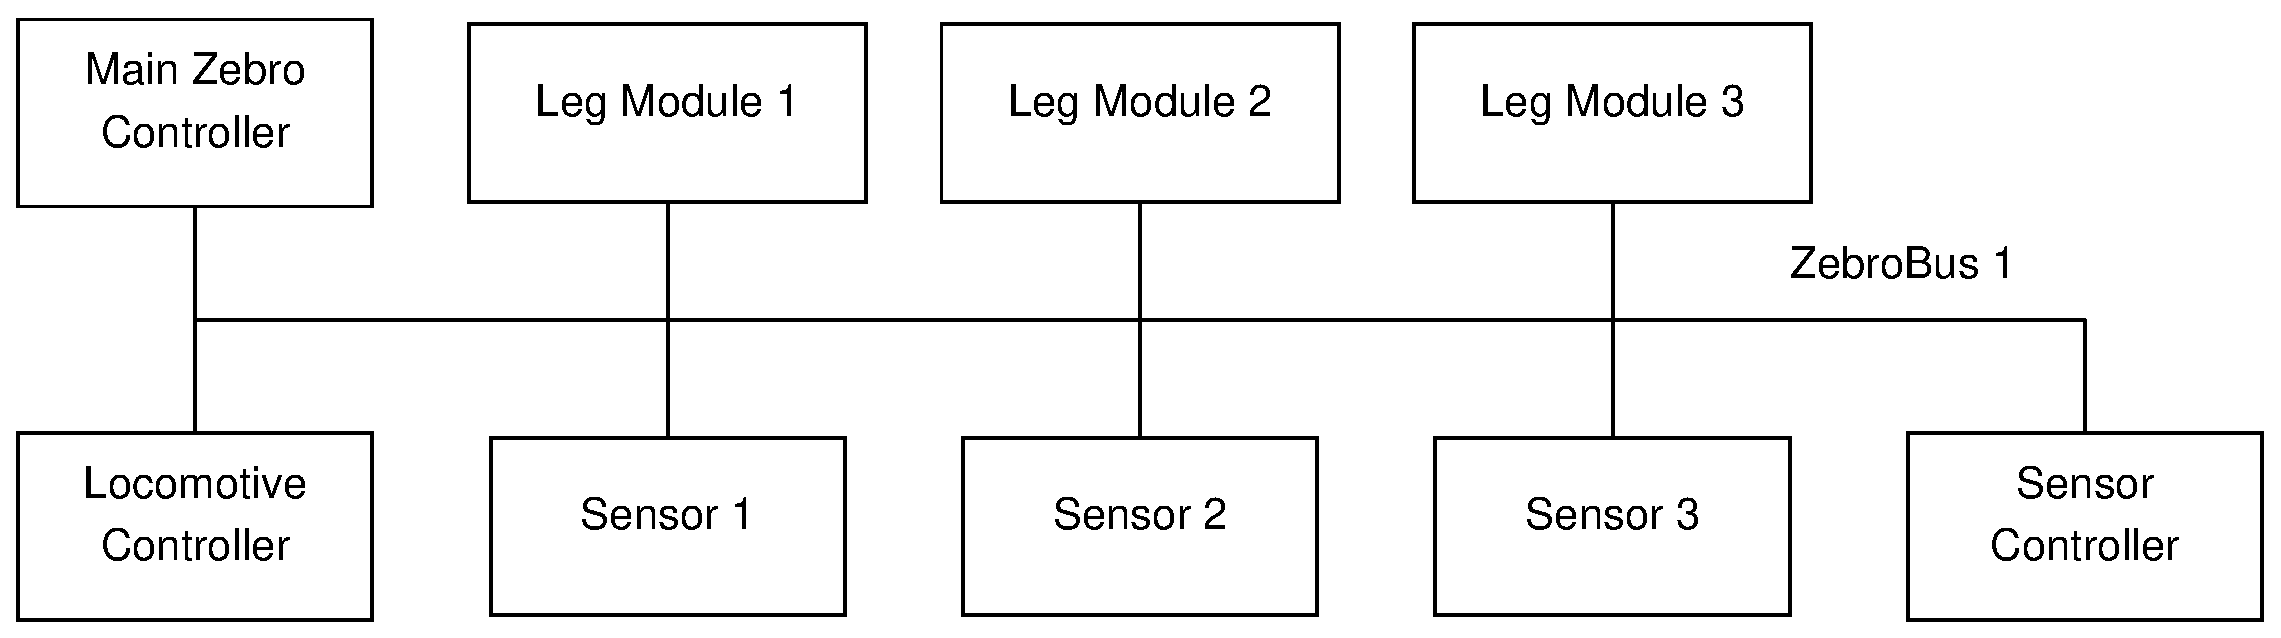
\includegraphics[scale=0.28]{fig/zebrobus_flat.eps}
                \caption{Flat hierarchy}
                \label{fig:ch3trace}     
        \end{subfigure}
        \begin{subfigure}[htpb]{\textwidth}
                \centering
                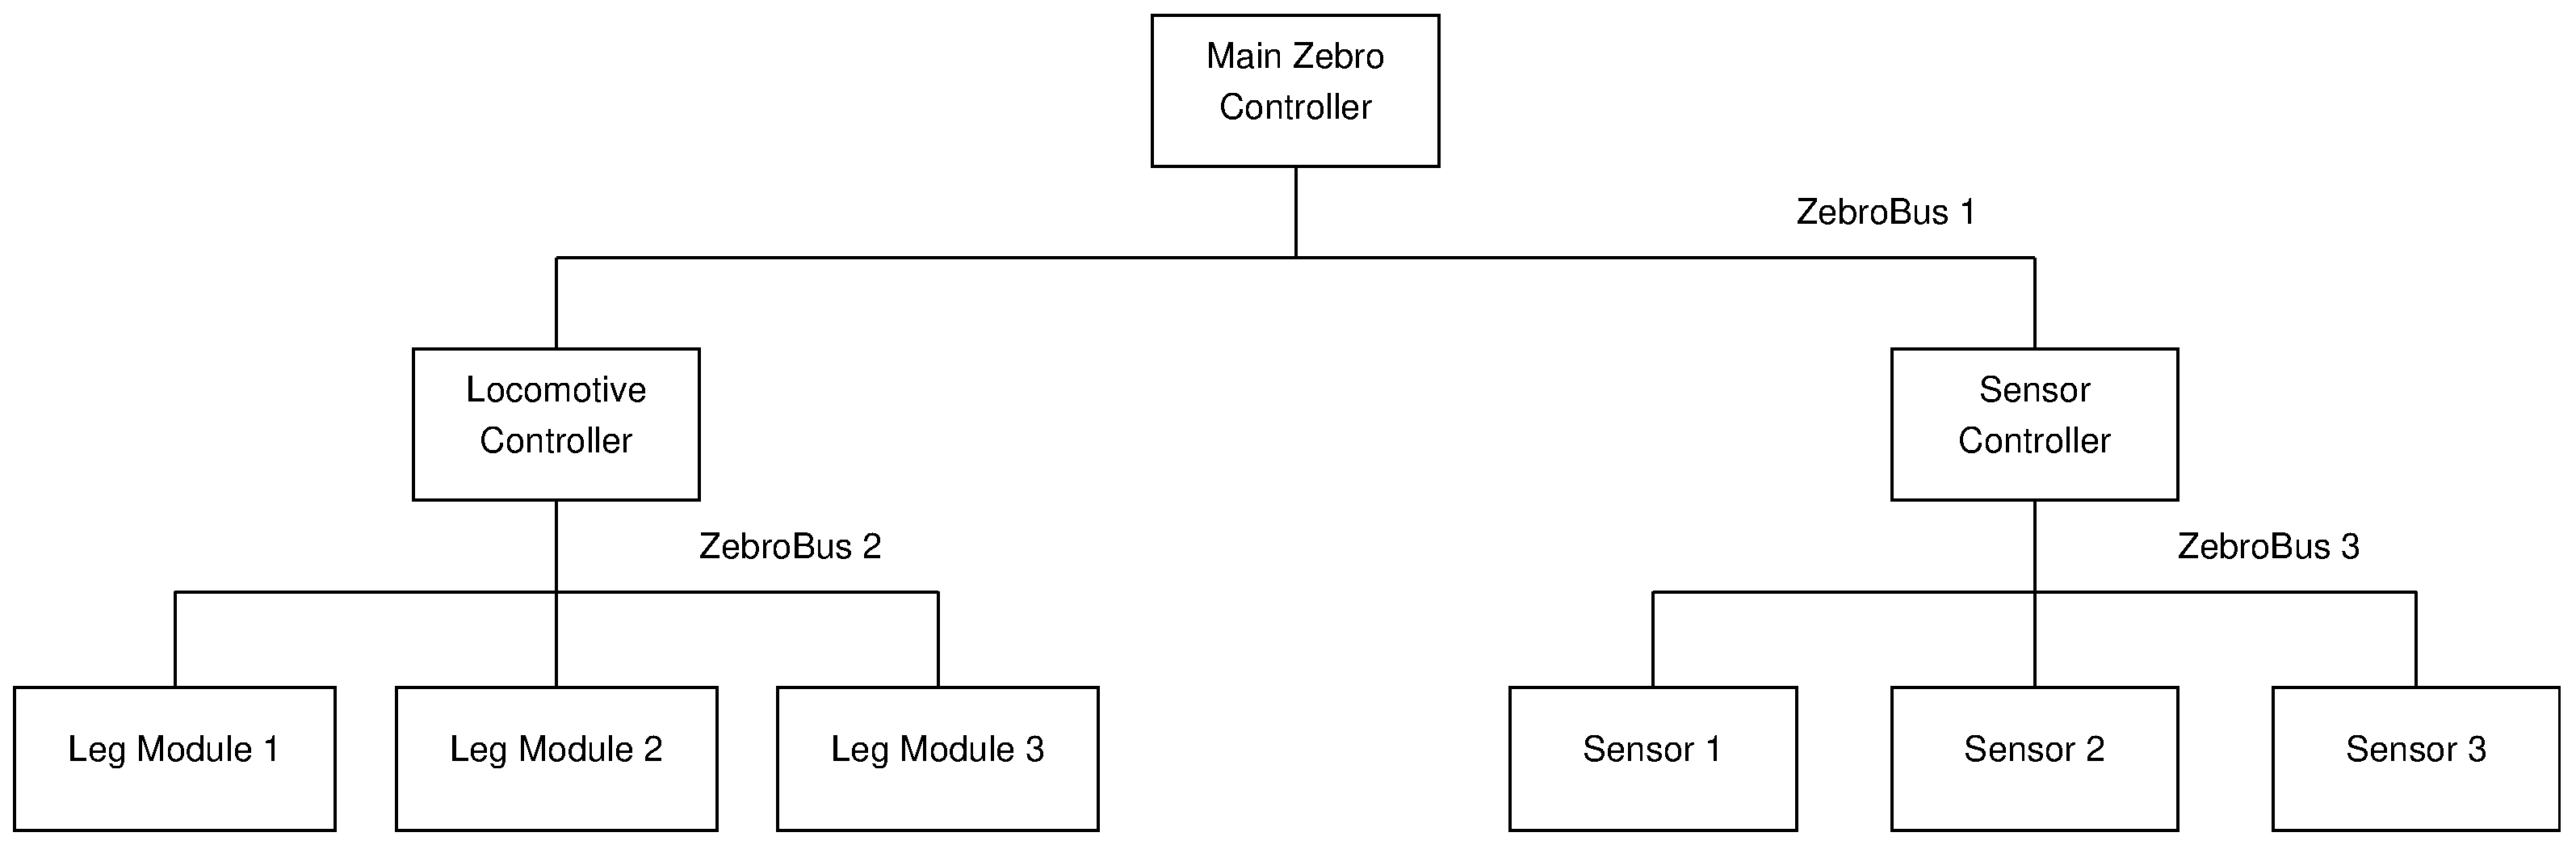
\includegraphics[scale=0.26]{fig/zebrobus_tree.eps}
                \caption{Tree hierarchy}
                \label{fig:ch3carPlotTree}
        \end{subfigure}
        \begin{subfigure}[htpb]{\textwidth}
        \centering
        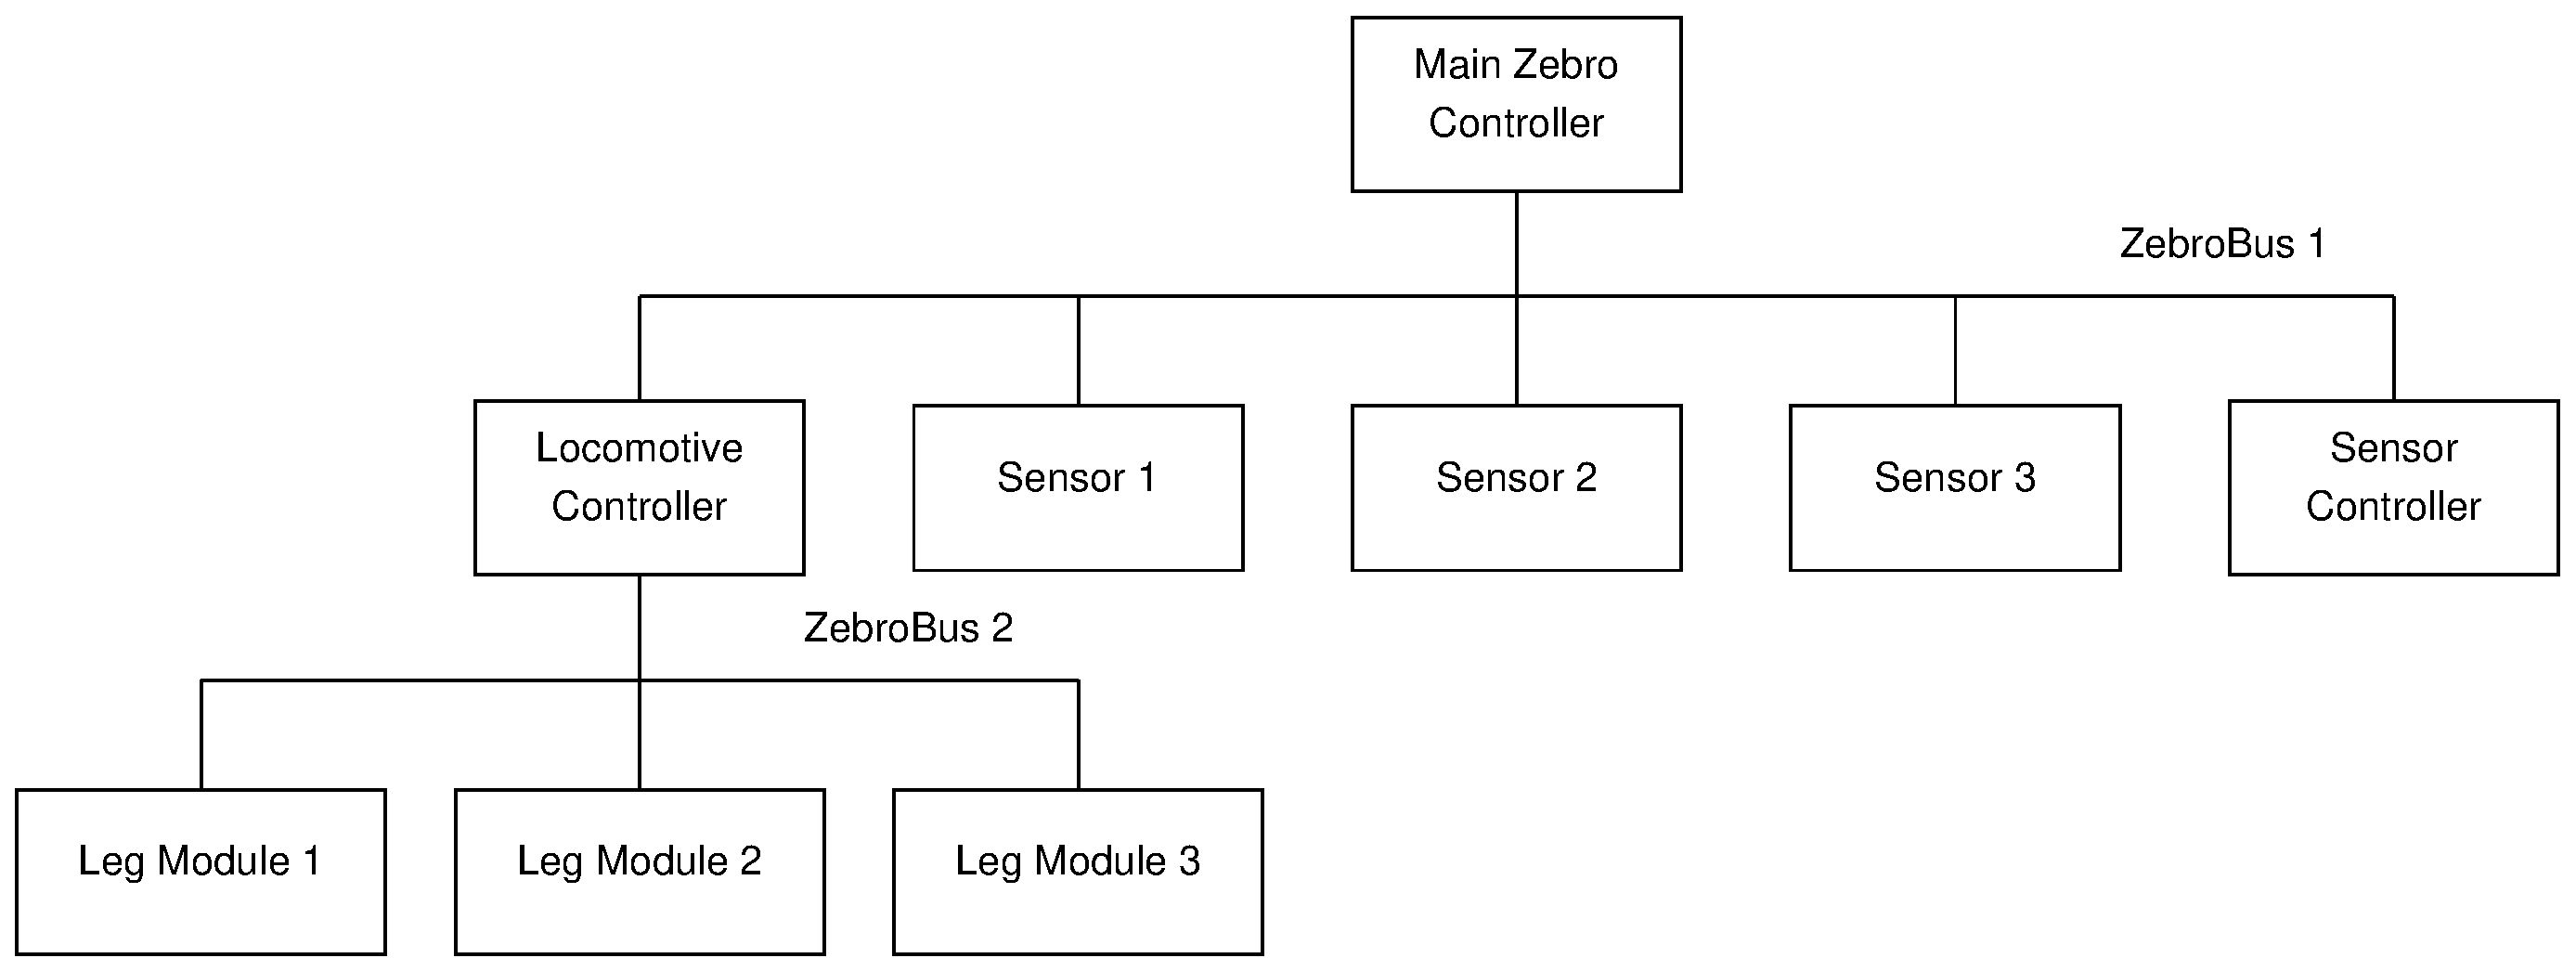
\includegraphics[scale=0.28]{fig/zebrobus_mixed.eps}
        \caption{Mixed hierarchy}
         \label{fig:ch3carPlotMixed}
        \end{subfigure}
        \caption{Schematic representation of different ZebroBus hierachies.}\label{fig:zebrobus_hierachies}
\end{figure}

\subsection{Bus address space and multicast}
ZebroBus uses 7 bit bus addresses, every device on the bus should have a unique bus address.

Some data should be received by more than one module on the bus.
One approach would be to transmit it to each of these devices individually, but this has two downsides.
Firstly, more resources are used. The master has to execute the transmission multiple times, and thus the bus is occupied for a longer period of time.
Secondly, not all modules receive the data at the same time. For time sensitive data, this can be a nuisance.
Therefore, ZebroBus reserves the lowest 16 bus addresses for multicast addresses. An overview of the bus address space is given in \cref{tab:bus_address_space}. No read requests should be send to a multicast address, and all read requests received on a multicast address should be ignored.
\begin{table}[H]
    \begin{center}
    \caption{Overview of the ZebroBus bus address space.}
    \label{tab:bus_address_space}
    \begin{tabular}{ll}
    \toprule
    Address & Name \\ \midrule
    0x00 -- 0x0F & multicast addresses \\
    0x10 -- 0x6F & device addresses \\
    0x70 -- 0x7F & reserved for future use \\
    \bottomrule
    \end{tabular}
    \end{center}
\end{table}

\subsection{Virtual registers}
A common convention used with I$^2$C interfaces is that data is transferred by first transmitting the register address of the data the masters wants to read or write on the slave, followed by the actual data.
This convention was followed for ZebroBus.
Every ZebroBus device should have a set of \emph{virtual registers} or \emph{vregs}, that have the following features:

\begin{enumerate}
\item The vregs are byte addressed
\item The vregs have 256 fields
\item When reading or writing more than one byte in a single I$^2$C transaction, the read or write register address should auto increment
\item After receiving the STOP bit, the read or write register address should be reset to the address that was last received.
\item The register address is shared for read and writes. i.e. the I$^2$C sequence \\
    \verb|START 0x31 0x42 0x43 STOP START READ_BYTE STOP| should do the following:
    \begin{enumerate}
        \item Write 0x42 to register address 0x31
        \item Write 0x43 to register address 0x32
        \item Read the value in register address 0x31
    \end{enumerate}
    However, it is considered good practise to always transmit the register address before performing a read.
\end{enumerate}
\section{Vregs fields}
There are four kinds of vregs fields, listed below.
Furthermore the fields at register addresses \verb|0xF0| through \verb|0xFF| are reserved for future use.

\begin{description}
\item[Shared]
    fields have the same function for all ZebroBus modules.
    They are located at register addresses \verb|0x00| through \verb|0x1F|.
    They are specified in \cref{sec:shared_fields}.
    
\item[Class specific]
    fields have the same function for all ZebroBus modules of the same class (e.g. leg modules, sensors, ...).
    They are located at register addresses \verb|0x20| through \verb|0x3F|.
    They are specified in  \cref{sec:class_specific_fields}.
    
\item[Device specific]
    fields may have a different function on every ZebroBus module.
    They are located at register addresses \verb|0x40| through \verb|0xEF|,
    and are not specified in this document.

\end{description}

Every vregs field contains a single 8-bit value.
When data spans multiple vregs fields, it should be stored most significant byte first and left aligned.
\subsection{Shared fields}\label{sec:shared_fields}
The functions of the shared fields are summarised in \cref{tab:shared_fields}.
For some fields a more detailed explanation is given below. Fields are always referenced by their register address.

\begin{description}

\item[Field 0x00 through 0x05]
    In this fields the value `0' is reserved.
    When used it means that this field is not implemented by the module.
    
    To explain the functionality of these fields, consider a leg module that supports up to ZebroBus version 1,
    is the second type of leg module to be designed, and the fifth design iteration on that type.
    Furthermore it is running the seventh version of the software for that iteration, and is the twelfth unit that was produced.
    
    Fields \verb|0x00| through \verb|0x05| should have the following values:
    \begin{description}
        \item[0x00 ZebroBus version:] 1, module the device supports up to ZebroBus version 1.
        \item[0x01 class id:] 1, because the module is a leg module.
        \item[0x02 product id:] 2, because it is the second type of leg module designed.
        \item[0x03 product version:] 5, because it is the fifth design of this type of leg module.
        \item[0x04 serial id:] 12, because it was the 12th unit produced
        \item[0x05 software version:] 7, because it is running the seventh version of the software.
    \end{description}
    
\item[serial id]
    It is possible to update the \verb|serial id| field over ZebroBus.
    In order to do so, the value \verb|1B| should be written to it, followed by the new value.
    
\item[quick status]
    should contain a one byte status message that a controller can use to quickly determine the state of
    a module.
    
\item[sync counter]
    This field is used for time synchronisation between different modules.
    The controller writes data to this address exactly once every second, the moment of this write can be used
    as a basis for all timing.
    Every time the controller writes a value to this register, it should increment that value. At \verb|0xFF| a roll over should occur.
    In this way every module can accurately determine the time modulo 256 seconds.
    This can be useful for synchronisation.
    
\item[loop counter]
    This field should contain a counter that the slave device increments every time it goes through its main control loop.
    If the slave device does not have a main control loop, this value should still be periodically incremented.

\item[error counter]
    This field should contain the number of errors that occurred in the slave device.
    When a write to this field occurs, the slave device should clear all errors.

\item[last error]
    This field should contain the code of the last error that occurred in the slave device
    
\end{description}

\begin{table}[H]
    \begin{center}
    \caption{Function of the shared vregs fields}
    \label{tab:shared_fields}
    \begin{tabularx}{\textwidth}{llllX}
    \toprule
    \multicolumn{2}{c}{Address} & Direction & Name & Description \\
    Dec & Hex &   &   \\
    \midrule
    0  & 00  & r   & ZebroBus version & Highest of the ZebroBus protocol supported \\
    1  & 01  & r   & class id         & Class this module is part of (e.g. leg module). See \cref{tab:zebrobus_classes} \\
    2  & 02  & r   & product id       & Product ID of this module\\
    3  & 03  & r   & product version  & Product version of this module \\
    4  & 04  & r/w & serial id        & Serial number of this module \\
    5  & 05  & r   & software version & Software version of this module \\
    6  & 06  & r   & zebrobus address & Primary ZebroBus slave address of this module \\
    7  & 07  & r    & reserved         & Reserved for future use \\
    ...  & ...  & r & reserved      & Reserved for future use \\
    16  & 0F  & r & reserved        & Reserved for future use \\
    17 & 10  & r   & quick status     & One byte module status message \\
    18 & 11  & r/w & sync counter     & Time synchronisation counter \\
    19 & 12  & r   & loop counter     & Counts the times we go through the main control loop \\
    20 & 13  & r/w & error counter    & Counts the number of errors that occurred \\
    21 & 14 & r    & last error        & Error code of the last error \\
    22 & 15  & r & reserved         & Reserved for future use  \\
    ... & ... & r & reserved        & Reserved for future use \\
    31 & 1F & r & reserved          & Reserved for future use \\
    \bottomrule
    \end{tabularx}
    \end{center}
\end{table}

\begin{table}[H]
    \begin{center}
    \caption{Overview of ZebroBus classes and there identifiers.}
    \label{tab:zebrobus_classes}
    \begin{tabular}{ll}
    \toprule
    ID & Name \\ \midrule
    0 & field not implemented \\
    1 & leg module \\
    2--255 & reserved for future use \\
    \bottomrule
    \end{tabular}
    \end{center}
\end{table}

\subsection{Class specific fields}\label{sec:class_specific_fields}
The Class specific fields should be shared by all modules with the same class id.
For each of the different classes a list of class specific fields is given below.
\subsubsection{Leg modules}
The class specific fields for leg modules are given in \cref{tab:class_leg_fields}.

The motion fields should behave as follows:
\begin{itemize}
    \item Fields \verb|0x20| through \verb|0x24| are buffered, meaning that
        data written to address \verb|0x20| through \verb|0x24| should only become active after data was written to \verb|motion update|.
    \item It does not matter what values gets written to \verb|motion update|.
    \item After writing to \verb|motion update|,
    the buffer values for fields \verb|0x20| through \verb|0x24| should be set to zero by the module.
    \item Reading from fields \verb|0x20| through \verb|0x24| should also read the active value.
    It is therefore not possible to read what values are in the buffer.
    \item \verb|motion crc| may contain a cyclic redundancy check (CRC) of fields \verb|0x20| through \verb|0x24|.
        When a slave does not implement this CRC, it can ignore the field.
        When a master does not implement this CRC, the field should be kept at `0'.
        In this version of the ZebroBus spec, the CRC polynomial is not yet specified.
    \item when \verb|sync counter| rolls over, the \verb|motion phase| field should be updated by the leg module in order to keep the motion continuous.
\end{itemize}

The motion speed field has units of 10 rpm. A speed of 1 means the leg should take 10 paces forward per minute.
A speed of -2 means it should take 20 paces backward a minute. 
Some speeds might be to high for the hardware used.
Speeds to high for hardware should be interpreted as the maximum possible speed by the leg module.\\
The motion phase field should be interpreted as the angle the leg would be at when the (synchronised) time was at 0.
The motion phase field should have a value between 0 and 239. When values 240-255 are written the leg should report an error and stop.
Because the leg unit can measure 24 evenly spaced angles on a circle precisely it was best to divide the circle in to a number of angles that is a multiple of 24.
When a time roll-over occurs the leg module updates the motion phase field to ensure a continuous movement. The relative phases between legs will not change on this time roll-over.


\begin{table}[H]
    \begin{center}
    \caption{Function of the class specific vregs fields for a leg module}
    \label{tab:class_leg_fields}
    \begin{tabularx}{\textwidth}{llllX}
    \toprule
    \multicolumn{2}{c}{Address} & Direction & Name & Description \\
    Dec & Hex &   &   \\
    \midrule
    32 & 20 & r/w & motion mode   & Predefined mode of action the leg module should execute see \cref{tab:leg_motion_modes} \\
    33 & 21 & r/w & motion speed  & Speed of the motion. Should be interpreted as a two's complement 8-bit value.\\
    34 & 22 & r/w & motion phase  & Phase offset of the motion.\\
    35 & 23 & r/w & motion extra  & Any extra information needed by the motion mode \\
    36 & 24 & r/w & motion crc    & Optional CRC of fields \verb|0x20| through \verb|0x23| \\
    37 & 25 & r/w & motion update & Activate the values written to  \verb|0x20| through \verb|0x24| \\
    38 & 26 & r/w & motor voltage & Nominal voltage of the installed motor. To write to this field,
                                    first the value \verb|67| should be written, followed by the actual value. 
                                    Value in volt.\\
    39 & 27 & r & reserved      & Reserved for future use \\
    ... & ... & r &  reserved    & Reserved for future use \\
    64 & 3F & r &  reserved      & Reserved for future use \\
    \bottomrule
    \end{tabularx}
    \end{center}
\end{table}

\begin{table}[H]
    \begin{center}
    \caption{Overview of ZebroBus leg module motion modes}
    \label{tab:leg_motion_modes}
    \begin{tabularx}{\textwidth}{llX}
    \toprule
    Value & Name & Description\\ \midrule
    0 & idle & Do nothing, just keep the leg where it is\\
    1 & walk & Regular forward walk.
                \verb|motion speed| determines the direction and speed of the walk.
                \verb|motion phase| determines the position the leg would have been
                            at the last time `0' was written to \verb|sync counter|\\
    2 & fixed position & Move the leg module to a fixed position.
                This position is determined by the \verb|motion phase| field.
                The speed and direction of the rotation to this position is determined by \verb|motion speed|\\
    3 & continuous rotation & Continuously rotate the leg.
                \verb|motion speed| determines the direction and speed of the rotation.
                \verb|motion phase| same as for `walk'. \\
    \bottomrule
    \end{tabularx}
    \end{center}
\end{table}


\end{document}
